% Draft for IEEE Robotics and Automation Letters (RA-L).
% Compiles with IEEEtran when the class is installed; otherwise falls back to a two-column
% article layout so the draft can be built anywhere. The body is identical in both cases.
% Every reported number is a macro from numbers.tex or a table from tables/, both generated by
% analysis/make_paper_numbers.py from the committed result files. Do not type results by hand.
\IfFileExists{IEEEtran.cls}{\documentclass[journal]{IEEEtran}}{\documentclass[10pt,twocolumn]{article}}
\makeatletter
\@ifclassloaded{IEEEtran}{}{%
  \usepackage[margin=0.72in,columnsep=0.25in]{geometry}
  \newenvironment{IEEEkeywords}{\par\smallskip\noindent\textbf{Index Terms---}\itshape}{\par}
  \newcommand{\IEEEPARstart}[2]{#1#2}
}
\makeatother
\usepackage[T1]{fontenc}
\usepackage{amsmath,amssymb}
\usepackage{booktabs}
\usepackage{graphicx}
\usepackage{xcolor}
\usepackage{url}
\graphicspath{{../figures/}}
% AUTO-GENERATED by analysis/make_paper_numbers.py from results/*.json. Do not edit.
\newcommand{\AgreeExp}{0.071}
\newcommand{\AgreeMax}{16}
\newcommand{\AgreeMean}{3.3}
\newcommand{\AgreeR}{0.56}
\newcommand{\AgreeRsq}{31}
\newcommand{\AgreeSD}{0.068}
\newcommand{\OneCanAMax}{0.96}
\newcommand{\OneCanAMean}{0.946}
\newcommand{\OneCanAMin}{0.90}
\newcommand{\OneCanARange}{6}
\newcommand{\OneCanASD}{0.023}
\newcommand{\OneCanASDcorr}{0.000}
\newcommand{\OneCanASDhi}{0.029}
\newcommand{\OneCanASDlo}{0.000}
\newcommand{\OneCanBFp}{0.453}
\newcommand{\OneCanBMeanHi}{0.95}
\newcommand{\OneCanBMeanLo}{0.89}
\newcommand{\OneCanBRange}{7}
\newcommand{\OneCanBRemlSDp}{0.004}
\newcommand{\OneCanBSDe}{0.046}
\newcommand{\OneCanBSDp}{0.004}
\newcommand{\OneCanBSDs}{0.025}
\newcommand{\OneCanBinom}{0.032}
\newcommand{\OneCanCFp}{0.184}
\newcommand{\OneCanCMeanHi}{0.96}
\newcommand{\OneCanCMeanLo}{0.86}
\newcommand{\OneCanCRange}{10}
\newcommand{\OneCanCRemlSDp}{0.025}
\newcommand{\OneCanCSDe}{0.045}
\newcommand{\OneCanCSDp}{0.024}
\newcommand{\OneCanCSDs}{0.000}
\newcommand{\OneCanD}{-0.58}
\newcommand{\OneCanDExHi}{0.44}
\newcommand{\OneCanDExLo}{-1.70}
\newcommand{\OneCanDExp}{0.7933}
\newcommand{\OneCanDExpHolm}{1.0000}
\newcommand{\OneCanDhi}{0.44}
\newcommand{\OneCanDlo}{-1.71}
\newcommand{\OneCanDp}{0.8010}
\newcommand{\OneCanDpHolm}{1.0000}
\newcommand{\OneCanDropBetter}{0.897}
\newcommand{\OneCanDropDiff}{4.7}
\newcommand{\OneCanDropP}{0.067}
\newcommand{\OneCanDropRest}{0.943}
\newcommand{\OneCanMDD}{3.7}
\newcommand{\OneCanMDDt}{5.3}
\newcommand{\OneCanMinDetF}{0.066}
\newcommand{\OneCanPowFour}{46}
\newcommand{\OneCanPowThree}{32}
\newcommand{\OneCanPowTwo}{4}
\newcommand{\OneCanR}{0.18}
\newcommand{\OneCanRCorr}{undefined}
\newcommand{\OneCanRCorrFloorFrac}{100}
\newcommand{\OneCanRCorrLo}{undefined}
\newcommand{\OneCanRExHi}{1.63}
\newcommand{\OneCanRExLo}{0.00}
\newcommand{\OneCanRExp}{0.880}
\newcommand{\OneCanRExpHolm}{1.000}
\newcommand{\OneCanRReml}{0.18}
\newcommand{\OneCanRhi}{1.64}
\newcommand{\OneCanRlo}{0.00}
\newcommand{\OneCanRp}{0.890}
\newcommand{\OneCanRpHolm}{1.000}
\newcommand{\OneCanTierBetween}{0.036}
\newcommand{\OneCanTierNull}{0.40}
\newcommand{\OneCanTierP}{0.200}
\newcommand{\OneCanTierShare}{0.82}
\newcommand{\OneCanTierWithin}{0.020}
\newcommand{\OneLiftAMax}{1.00}
\newcommand{\OneLiftAMean}{0.988}
\newcommand{\OneLiftAMin}{0.96}
\newcommand{\OneLiftARange}{4}
\newcommand{\OneLiftASD}{0.017}
\newcommand{\OneLiftASDcorr}{0.007}
\newcommand{\OneLiftASDhi}{0.020}
\newcommand{\OneLiftASDlo}{0.006}
\newcommand{\OneLiftBFp}{0.094}
\newcommand{\OneLiftBMeanHi}{1.00}
\newcommand{\OneLiftBMeanLo}{0.97}
\newcommand{\OneLiftBRange}{3}
\newcommand{\OneLiftBRemlSDp}{0.012}
\newcommand{\OneLiftBSDe}{0.015}
\newcommand{\OneLiftBSDp}{0.011}
\newcommand{\OneLiftBSDs}{0.000}
\newcommand{\OneLiftBinom}{0.015}
\newcommand{\OneLiftCFp}{0.479}
\newcommand{\OneLiftCMeanHi}{0.99}
\newcommand{\OneLiftCMeanLo}{0.93}
\newcommand{\OneLiftCRange}{7}
\newcommand{\OneLiftCRemlSDp}{0.000}
\newcommand{\OneLiftCSDe}{0.043}
\newcommand{\OneLiftCSDp}{0.000}
\newcommand{\OneLiftCSDs}{0.000}
\newcommand{\OneLiftD}{0.12}
\newcommand{\OneLiftDExHi}{0.25}
\newcommand{\OneLiftDExLo}{-0.15}
\newcommand{\OneLiftDExp}{0.1937}
\newcommand{\OneLiftDExpHolm}{0.9684}
\newcommand{\OneLiftDhi}{0.25}
\newcommand{\OneLiftDlo}{-0.15}
\newcommand{\OneLiftDp}{0.1880}
\newcommand{\OneLiftDpHolm}{0.9400}
\newcommand{\OneLiftDropBetter}{0.973}
\newcommand{\OneLiftDropDiff}{1.8}
\newcommand{\OneLiftDropP}{0.133}
\newcommand{\OneLiftDropRest}{0.992}
\newcommand{\OneLiftMDD}{2.7}
\newcommand{\OneLiftMDDt}{3.8}
\newcommand{\OneLiftMinDetF}{0.022}
\newcommand{\OneLiftPowFour}{60}
\newcommand{\OneLiftPowThree}{38}
\newcommand{\OneLiftPowTwo}{16}
\newcommand{\OneLiftR}{0.66}
\newcommand{\OneLiftRCorr}{1.62}
\newcommand{\OneLiftRCorrFloorFrac}{35}
\newcommand{\OneLiftRCorrLo}{0.00}
\newcommand{\OneLiftRExHi}{1.52}
\newcommand{\OneLiftRExLo}{0.00}
\newcommand{\OneLiftRExp}{0.893}
\newcommand{\OneLiftRExpHolm}{1.000}
\newcommand{\OneLiftRReml}{0.69}
\newcommand{\OneLiftRhi}{1.35}
\newcommand{\OneLiftRlo}{0.00}
\newcommand{\OneLiftRp}{0.898}
\newcommand{\OneLiftRpHolm}{1.000}
\newcommand{\OneLiftTierBetween}{0.018}
\newcommand{\OneLiftTierNull}{0.40}
\newcommand{\OneLiftTierP}{0.467}
\newcommand{\OneLiftTierShare}{0.54}
\newcommand{\OneLiftTierWithin}{0.016}
\newcommand{\OneSqAMax}{0.72}
\newcommand{\OneSqAMean}{0.600}
\newcommand{\OneSqAMin}{0.50}
\newcommand{\OneSqARange}{22}
\newcommand{\OneSqASD}{0.079}
\newcommand{\OneSqASDcorr}{0.039}
\newcommand{\OneSqASDhi}{0.096}
\newcommand{\OneSqASDlo}{0.044}
\newcommand{\OneSqBFp}{0.003}
\newcommand{\OneSqBMeanHi}{0.68}
\newcommand{\OneSqBMeanLo}{0.45}
\newcommand{\OneSqBRange}{23}
\newcommand{\OneSqBRemlSDp}{0.086}
\newcommand{\OneSqBSDe}{0.057}
\newcommand{\OneSqBSDp}{0.086}
\newcommand{\OneSqBSDs}{0.027}
\newcommand{\OneSqBinom}{0.069}
\newcommand{\OneSqCFp}{0.121}
\newcommand{\OneSqCMeanHi}{0.66}
\newcommand{\OneSqCMeanLo}{0.53}
\newcommand{\OneSqCRange}{13}
\newcommand{\OneSqCRemlSDp}{0.033}
\newcommand{\OneSqCSDe}{0.050}
\newcommand{\OneSqCSDp}{0.033}
\newcommand{\OneSqCSDs}{0.007}
\newcommand{\OneSqD}{6.22}
\newcommand{\OneSqDExHi}{10.49}
\newcommand{\OneSqDExLo}{-1.35}
\newcommand{\OneSqDExp}{0.0844}
\newcommand{\OneSqDExpHolm}{0.5062}
\newcommand{\OneSqDhi}{10.74}
\newcommand{\OneSqDlo}{-1.35}
\newcommand{\OneSqDp}{0.0810}
\newcommand{\OneSqDpHolm}{0.4860}
\newcommand{\OneSqDropBOne}{0.493}
\newcommand{\OneSqDropBTwo}{0.453}
\newcommand{\OneSqDropBetter}{0.473}
\newcommand{\OneSqDropDiff}{17.2}
\newcommand{\OneSqDropOOne}{0.620}
\newcommand{\OneSqDropOTwo}{0.680}
\newcommand{\OneSqDropP}{0.067}
\newcommand{\OneSqDropRest}{0.645}
\newcommand{\OneSqDropWOne}{0.647}
\newcommand{\OneSqDropWTwo}{0.633}
\newcommand{\OneSqMDD}{12.7}
\newcommand{\OneSqMDDt}{18.0}
\newcommand{\OneSqMinDetF}{0.083}
\newcommand{\OneSqPowFour}{66}
\newcommand{\OneSqPowThree}{42}
\newcommand{\OneSqPowTwo}{18}
\newcommand{\OneSqR}{1.08}
\newcommand{\OneSqRCorr}{2.20}
\newcommand{\OneSqRCorrFloorFrac}{32}
\newcommand{\OneSqRCorrLo}{0.00}
\newcommand{\OneSqRExHi}{1.93}
\newcommand{\OneSqRExLo}{0.00}
\newcommand{\OneSqRExp}{0.427}
\newcommand{\OneSqRExpHolm}{1.000}
\newcommand{\OneSqRReml}{1.08}
\newcommand{\OneSqRhi}{1.84}
\newcommand{\OneSqRlo}{0.00}
\newcommand{\OneSqRp}{0.442}
\newcommand{\OneSqRpHolm}{1.000}
\newcommand{\OneSqTierBetween}{0.124}
\newcommand{\OneSqTierNull}{0.40}
\newcommand{\OneSqTierP}{0.200}
\newcommand{\OneSqTierShare}{0.94}
\newcommand{\OneSqTierWithin}{0.038}
\newcommand{\TwoSqAMax}{0.69}
\newcommand{\TwoSqAMean}{0.639}
\newcommand{\TwoSqAMin}{0.59}
\newcommand{\TwoSqARange}{10}
\newcommand{\TwoSqASD}{0.031}
\newcommand{\TwoSqASDcorr}{0.023}
\newcommand{\TwoSqASDhi}{0.039}
\newcommand{\TwoSqASDlo}{0.017}
\newcommand{\TwoSqBFp}{0.012}
\newcommand{\TwoSqBMeanHi}{0.72}
\newcommand{\TwoSqBMeanLo}{0.54}
\newcommand{\TwoSqBRange}{18}
\newcommand{\TwoSqBRemlSDp}{0.054}
\newcommand{\TwoSqBSDe}{0.045}
\newcommand{\TwoSqBSDp}{0.054}
\newcommand{\TwoSqBSDs}{0.000}
\newcommand{\TwoSqBinom}{0.021}
\newcommand{\TwoSqCFp}{0.349}
\newcommand{\TwoSqCMeanHi}{0.66}
\newcommand{\TwoSqCMeanLo}{0.59}
\newcommand{\TwoSqCRange}{7}
\newcommand{\TwoSqCRemlSDp}{0.014}
\newcommand{\TwoSqCSDe}{0.045}
\newcommand{\TwoSqCSDp}{0.014}
\newcommand{\TwoSqCSDs}{0.010}
\newcommand{\TwoSqD}{2.69}
\newcommand{\TwoSqDExHi}{5.23}
\newcommand{\TwoSqDExLo}{-0.00}
\newcommand{\TwoSqDExp}{0.0251}
\newcommand{\TwoSqDExpHolm}{0.0501}
\newcommand{\TwoSqDhi}{5.12}
\newcommand{\TwoSqDlo}{0.02}
\newcommand{\TwoSqDp}{0.0245}
\newcommand{\TwoSqDpHolm}{0.0490}
\newcommand{\TwoSqDropBOne}{0.624}
\newcommand{\TwoSqDropBTwo}{0.539}
\newcommand{\TwoSqDropBetter}{0.581}
\newcommand{\TwoSqDropDiff}{7.5}
\newcommand{\TwoSqDropOOne}{0.607}
\newcommand{\TwoSqDropOTwo}{0.716}
\newcommand{\TwoSqDropP}{0.133}
\newcommand{\TwoSqDropRest}{0.656}
\newcommand{\TwoSqDropWOne}{0.667}
\newcommand{\TwoSqDropWTwo}{0.635}
\newcommand{\TwoSqMDD}{5.0}
\newcommand{\TwoSqMDDt}{7.1}
\newcommand{\TwoSqMinDetF}{0.065}
\newcommand{\TwoSqPowFour}{52}
\newcommand{\TwoSqPowThree}{32}
\newcommand{\TwoSqPowTwo}{13}
\newcommand{\TwoSqR}{1.71}
\newcommand{\TwoSqRCorr}{2.36}
\newcommand{\TwoSqRCorrFloorFrac}{10}
\newcommand{\TwoSqRCorrLo}{0.68}
\newcommand{\TwoSqRExHi}{3.18}
\newcommand{\TwoSqRExLo}{0.52}
\newcommand{\TwoSqRExp}{0.126}
\newcommand{\TwoSqRExpHolm}{0.126}
\newcommand{\TwoSqRReml}{1.74}
\newcommand{\TwoSqRhi}{2.96}
\newcommand{\TwoSqRlo}{0.51}
\newcommand{\TwoSqRp}{0.115}
\newcommand{\TwoSqRpHolm}{0.115}
\newcommand{\TwoSqTierBetween}{0.071}
\newcommand{\TwoSqTierNull}{0.40}
\newcommand{\TwoSqTierP}{0.467}
\newcommand{\TwoSqTierShare}{0.43}
\newcommand{\TwoSqTierWithin}{0.075}


\newcommand{\sdp}{\hat\sigma_p}
\newcommand{\sds}{\hat\sigma_s}
\newcommand{\sde}{\hat\sigma_e}

\begin{document}

\title{What Can Three Seeds and Fifty Rollouts Resolve?\\ A Preregistered Audit of Operator and Seed Variance on robomimic Multi-Human Benchmarks}

\author{Jaiveer Bassi%
\thanks{J. Bassi is an independent researcher (e-mail: jaiveerbassi@yahoo.com).}%
\thanks{Code, preregistration, partitions, initial states, per-run and per-rollout results: \protect\url{https://github.com/imjbassi/operator-variance-audit}.}}

\maketitle

\begin{abstract}
Results on the robomimic Multi-Human (MH) imitation-learning benchmarks are conventionally reported as a mean over three training seeds, each evaluated with 50 rollouts. We preregistered the hypothesis that the variance caused by \emph{which operators' demonstrations are in the training set} exceeds the variance caused by training seed, and tested it with 138 BC-RNN training runs on Lift, Can and Square: ten seeds at fixed data, six leave-one-operator-out partitions, and six size-matched random partitions as a control, all evaluated at the final checkpoint on fixed initial states. The preregistered tests were not met on any task, and we report that negative result with its power: with six operators the procedure detects a true ratio of two only \OneSqPowTwo\% of the time. What the data do establish concerns the reporting convention itself. On Lift and Can the spread across seeds is indistinguishable from the binomial noise of a single 50-rollout estimate. On Square, two three-seed means must differ by \OneSqMDD{} points to be distinguished. Re-evaluating the same 46 Square checkpoints with 500 rollouts, the 50-rollout success rates correlate only $r=\AgreeR$ with the 500-rollout ones, and an apparent proficiency-tier pattern (between-tier share \OneSqTierShare) disappears (\TwoSqTierShare). At 500 rollouts the operator-partition standard deviation is \TwoSqBSDp{} against \TwoSqCSDp{} for random partitions, a contrast that sits exactly at the decision boundary and that we do not claim. We give concrete reporting recommendations.
\end{abstract}

\begin{IEEEkeywords}
Imitation learning, benchmarking, reproducibility, variance components, learning from demonstration.
\end{IEEEkeywords}

\section{Introduction}
\IEEEPARstart{T}{he} robomimic study~\cite{mandlekar2021robomimic} established the most widely used protocol for evaluating offline imitation learning in manipulation: train on a fixed demonstration dataset, evaluate with 50 rollouts, and report success rate averaged over three seeds. Its Multi-Human (MH) datasets, 300 demonstrations per task from six operators of varied proficiency collected with RoboTurk~\cite{mandlekar2018roboturk}, are a standard testbed, and later work reports on them with the same three training seeds and 50 evaluation episodes, for example Diffusion Policy and the baselines it compares against~\cite{chi2023diffusion}. The three-seed standard deviation is the only uncertainty attached to such numbers.

A three-seed standard deviation measures one thing: how much the result moves when the optimizer's random stream changes and everything else is held fixed. It says nothing about how much the result would move had the dataset contained different demonstrations, or demonstrations from different people. For a benchmark built from six operators, that second source is not obviously smaller than the first. If it is larger, the conventional uncertainty understates the real one, and comparisons separated by a few points are not resolvable from the reported statistic.

We set out to test that claim directly and preregistered it before any training run. The claim, as preregistered, was not supported. This paper reports that outcome plainly, and then reports what the experiment did establish, which is a statement about the measurement rather than about operators:
\begin{itemize}
\item \textbf{A preregistered negative result with its power.} On no task does the operator-partition standard deviation exceed the seed standard deviation with an interval excluding one, nor does it exceed the matched random-partition control with an interval excluding zero (Section~\ref{sec:primary}). With six operators the preregistered procedure has \OneSqPowTwo\% power at a true ratio of two and \OneSqPowThree\% at three, so the negative result bounds little.
\item \textbf{The seed spread is mostly evaluation noise.} On Lift and Can the across-seed standard deviation of a 50-rollout success rate is indistinguishable from the binomial noise of one such estimate. On Square it is \OneSqASD{} against a floor of \OneSqBinom{} (Section~\ref{sec:floor}).
\item \textbf{Fifty rollouts do not characterise a checkpoint.} Re-evaluating the same 46 Square checkpoints with 500 rollouts, the 50-rollout numbers explain \AgreeRsq\% of the variance of the 500-rollout numbers, and a tier pattern that looked strong at 50 rollouts is absent at 500 (Section~\ref{sec:stage2}).
\item \textbf{A resolvability table.} We give the smallest difference between two three-seed means that the convention can resolve on each task (Section~\ref{sec:resolve}), and recommendations that follow (Section~\ref{sec:recs}).
\end{itemize}
We cite robomimic as the origin of a convention that the field, including this author, has used; nothing here is a criticism of that study, which also released the per-operator labels that make this audit possible.

\section{Related Work}
\textbf{Seeds and statistical practice.} That deep reinforcement learning results vary strongly with seed, and that small seed counts make comparisons unreliable, is well documented~\cite{henderson2018matters,colas2018seeds,agarwal2021precipice}. Bouthillier \emph{et al.}~\cite{bouthillier2021variance} showed for supervised benchmarks that variance from data sampling, parameter initialisation and hyperparameter choice all markedly affect comparisons, and that estimators which account for more of these sources are more reliable; our Arm~C is the imitation-learning analogue of their data-resampling source. For robot learning, Kress-Gazit \emph{et al.}~\cite{kressgazit2024empirical} recommend reporting evaluation conditions and statistical uncertainty in detail. We add a measurement, on a specific and heavily used benchmark, of how the conventional statistic decomposes.

\textbf{Demonstrator heterogeneity.} The robomimic study analysed MH data by proficiency tier, pooling the two operators in each tier, to ask how algorithms cope with suboptimal data~\cite{mandlekar2021robomimic}. Individual operators were not a unit of analysis there. Data quality and the compatibility of demonstrations from different people are known to affect imitation learning~\cite{belkhale2023dataquality,gandhi2022compatible}. Our question is narrower and statistical: treating the operator as the unit of replication, how much does benchmark performance move when one operator is removed, relative to seed and to removing the same number of random demonstrations?

\textbf{Preregistration.} Fixing hypotheses and analyses before data collection separates confirmatory from exploratory findings~\cite{nosek2018prereg}. We follow that practice, including a dated amendment log, and keep the distinction explicit throughout.

\section{Preregistered Design}
\label{sec:design}
The preregistration, with predictions, falsification criteria, the analysis plan and three dated amendments, was committed to the public repository before any training run and is reproduced there unchanged.

\subsection{Data and operator identity}
We use the robomimic v1.5 MH low-dimensional datasets for Lift, Can and Square (robosuite~\cite{zhu2020robosuite} 1.5.1). Each has 300 demonstrations, 50 from each of six operators. Operator identity is read directly from the filter keys shipped in the files (\texttt{better\_operator\_1}, \dots, \texttt{worse\_operator\_2}); we verified that the six keys are disjoint, each holds 50 contiguous demonstrations, and their union is the full dataset. No inference of identity is involved. The operator index is defined within a tier, and whether a given label denotes the same person across tasks is not documented, so we make no cross-task statement about individuals.

\subsection{Policy, training and evaluation}
All runs train BC-RNN with the robomimic low-dimensional hyperparameters: a two-layer LSTM of width 400 with a five-mode Gaussian-mixture head, sequence length 10, Adam with learning rate $10^{-4}$, batch size 100, and 2000 epochs of 100 gradient steps (robomimic v0.5.0). We evaluate only the \emph{final} checkpoint. The original study reports the maximum success rate over periodic evaluations during training and notes that other selection rules give lower numbers~\cite{mandlekar2021robomimic}; selecting on the evaluation rollouts is selection on the test set, so no selection is performed here. Our final-checkpoint means on the full datasets are \OneLiftAMean, \OneCanAMean{} and \OneSqAMean. For reference, the maximum-over-training figures reported in~\cite[Table~1]{mandlekar2021robomimic} for BC-RNN on the original MH low-dimensional datasets are 100.0, 100.0 and 78.0; the two sets of numbers differ in checkpoint rule and dataset version and are not directly comparable.
% Table 1 values (BC-RNN, low-dim, MH: 100.0 +- 0.0, 100.0 +- 0.0, 78.0 +- 4.3) were read twice from the ar5iv HTML of arXiv:2108.03298 on 2026-10-01.

Each checkpoint is evaluated with 50 rollouts of horizon 500 on 50 initial conditions that are generated once per task from seeded resets, stored, and reused for every checkpoint. Because robosuite regenerates the scene model at each reset and Lift randomises the cube size, both the simulator state and the model description are stored and restored. The rollout random stream is also fixed per rollout index. Evaluation is repeatable: re-running a checkpoint on the stored conditions reproduced every rollout outcome and step count in our check.

\subsection{Three arms}
\textbf{Arm A (seed).} All 300 demonstrations, ten seeds: 10 runs per task.

\textbf{Arm B (operator composition).} Six leave-one-operator-out partitions of 250 demonstrations, three seeds each: 18 runs per task. All partitions have the same size with no subsampling.

\textbf{Arm C (matched random control).} Six partitions of 250 demonstrations drawn uniformly at random from the 300, ignoring operators, three seeds each: 18 runs per task.

Arm~C is load-bearing. Two Arm~B partitions differ in which operator is absent, but also simply in which demonstrations are present; any two of them share 200 of their 250 demonstrations. Arm~C partitions have the same size and a comparable overlap, and isolate the second effect. If the spread across Arm~B partitions does not exceed the spread across Arm~C partitions, an operator effect is not separable from demonstration resampling at this sample size. Partition memberships were generated once, committed, and never changed. In total there are 138 training runs and 6{,}900 evaluation rollouts.

\subsection{Statistics}
\label{sec:stats}
The unit of replication is the operator (equivalently, the partition), never the rollout or the demonstration. The per-run statistic is the success rate $y$ of the final checkpoint.

\emph{Seed spread.} For Arm~A we report the sample standard deviation over the ten seeds, $s_A$, with a seed-bootstrap interval. Note that $s_A$ is the spread of \emph{measured} success rates and therefore includes the binomial noise of a finite number of rollouts, $\sqrt{\bar p(1-\bar p)/n}$.

\emph{Variance components.} For Arms~B and~C separately, the $6\times 3$ table of partitions $p$ by seeds $s$ is modelled as
\begin{equation}
y_{ps} = \mu + a_p + b_s + e_{ps},
\end{equation}
with independent zero-mean effects of variance $\sigma_p^2$, $\sigma_s^2$ and $\sigma_e^2$. We estimate the components by the method of moments, $\hat\sigma_p^2=(\mathrm{MS}_p-\mathrm{MS}_e)/3$ and $\hat\sigma_s^2=(\mathrm{MS}_s-\mathrm{MS}_e)/6$, truncated at zero~\cite{searle1992variance}, and, as a second estimator, by REML~\cite{patterson1971reml} in a crossed mixed model~\cite{seabold2010statsmodels}. The residual absorbs rollout noise and any partition-by-seed interaction. An estimate of exactly zero is a boundary estimate and is marked as such; it is not evidence that the variance is zero.

\emph{Headline ratio.} $R=\sdp^{B}/s_A$, with a 95\% percentile interval from a joint bootstrap~\cite{efron1993bootstrap} that resamples the six partitions and the ten Arm~A seeds with replacement (2000 resamples). The claim is supported for a task if the interval excludes~1.

\emph{Control contrast.} $D=(\sdp^{B})^2-(\sdp^{C})^2$, with a bootstrap over the six partitions of each arm. An operator effect is declared separable only if the interval excludes~0.

\emph{Multiple comparisons.} The primary family is six contrasts, $R>1$ and $D>0$ on three tasks, corrected by Holm's procedure~\cite{holm1979}. Raw and corrected one-sided $p$-values are reported.

\emph{Secondary claim.} Tier labels were predicted not to capture the operator effect. We decompose the between-partition sum of squares of the Arm~B partition means into between-tier and within-tier parts and compare the between-tier share to its distribution under relabelling.

\subsection{Amendments}
\label{sec:amend}
\emph{Amendment 1} was made before any data existed, after tests of the analysis code on synthetic tables. It records that the tier permutation test has only 15 distinct outcomes, so its $p$-value cannot fall below $1/15$ and the secondary claim must be judged by effect size; and that power would be reported by simulating the actual headline procedure, which synthetic runs had shown to be weak with six groups.

\emph{Amendment 2} was written after all Stage~1 results were seen and before any further rollout. Stage~1 showed that rollout noise was as large as the quantities being compared. Amendment~2 specifies a follow-up, \emph{Stage~2}: the 46 existing Square final checkpoints are re-evaluated with 500 rollouts each on 500 new fixed initial conditions, and the same analysis is applied unchanged, with a two-contrast Holm family. Stage~2 reuses the Stage~1 checkpoints, was designed after seeing Stage~1, and is therefore a follow-up rather than independent confirmation. It also declares three analyses exploratory (Section~\ref{sec:explore}).

\emph{Amendment 3} records the Stage~2 outcome and two reporting corrections described in Sections~\ref{sec:stage2} and~\ref{sec:tier}.

\begin{figure*}[t]
\centering
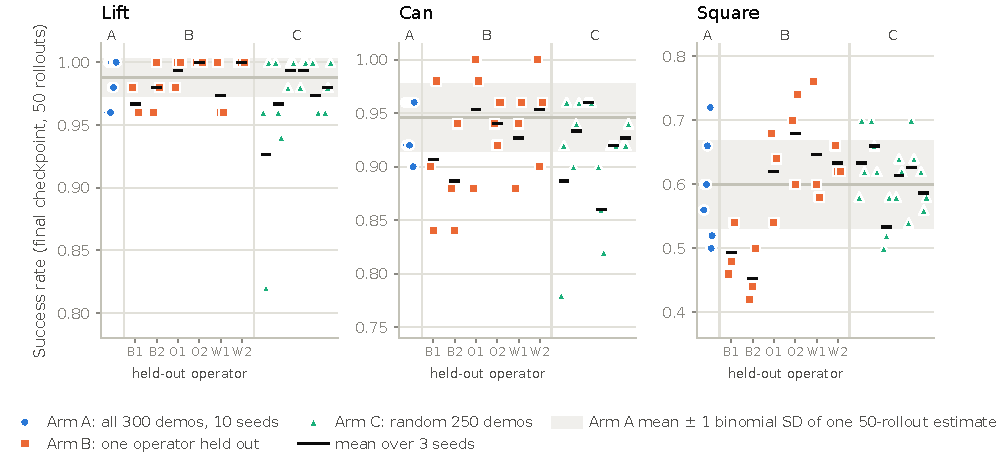
\includegraphics[width=\textwidth]{fig_arms.pdf}
\caption{Stage~1. Final-checkpoint success rate of every run (50 rollouts each). A: ten seeds on all 300 demonstrations. B: six leave-one-operator-out partitions, three seeds each, labelled by the held-out operator (B/O/W: better/okay/worse tier). C: six random 250-demonstration partitions, three seeds each. Bars are three-seed means. The grey band is the Arm~A mean $\pm$ one binomial standard deviation of a single 50-rollout estimate. Note the different vertical scales.}
\label{fig:arms}
\end{figure*}

\begin{table*}[t]
\centering
\caption{Variance components (method of moments; REML agrees to within 0.003 on every entry) and the preregistered contrasts. ``Floor'' is the binomial SD of one estimate at the Arm~A mean. $R=\sdp^{B}/s_A$; $D=(\sdp^{B})^2-(\sdp^{C})^2$. Intervals are 95\% bootstrap intervals from the preregistered 2000 resamples. For $D$, $p$-values are given as preregistered resampling / exact enumeration. $^{\dagger}$Boundary estimate (truncated at zero), not evidence of zero variance.}
\label{tab:components}
\setlength{\tabcolsep}{3.2pt}
\resizebox{\textwidth}{!}{% AUTO-GENERATED by analysis/make_paper_numbers.py. Do not edit.
\begin{tabular}{@{}l ccc ccc ccc cc ccc@{}}
\toprule
 & \multicolumn{3}{c}{Arm A (10 seeds)} & \multicolumn{3}{c}{Arm B (operator held out)} & \multicolumn{3}{c}{Arm C (random 250)} & \multicolumn{2}{c}{$R$ (Sec.~\ref{sec:stats})} & \multicolumn{3}{c}{$D \times 10^{3}$ (Sec.~\ref{sec:stats})} \\
\cmidrule(lr){2-4}\cmidrule(lr){5-7}\cmidrule(lr){8-10}\cmidrule(lr){11-12}\cmidrule(l){13-15}
Task & mean & SD & floor & $\hat\sigma_p$ & $\hat\sigma_s$ & $\hat\sigma_e$ & $\hat\sigma_p$ & $\hat\sigma_s$ & $\hat\sigma_e$ & est.\ [95\%] & $p_{\mathrm{Holm}}$ & est.\ [95\%] & $p$ & $p_{\mathrm{Holm}}$ \\
\midrule
\multicolumn{15}{@{}l}{\emph{Stage 1 (preregistered primary): 50 rollouts per checkpoint}} \\
Lift & 0.988 & 0.017 & 0.015 & 0.011 & 0.000$^{\dagger}$ & 0.015 & 0.000$^{\dagger}$ & 0.000$^{\dagger}$ & 0.043 & 0.66 [0.00, 1.35] & 1.000 & 0.12 [-0.15, 0.25] & 0.1880 / 0.1937 & 0.9400 / 0.9684 \\
Can & 0.946 & 0.023 & 0.032 & 0.004 & 0.025 & 0.046 & 0.024 & 0.000$^{\dagger}$ & 0.045 & 0.18 [0.00, 1.64] & 1.000 & -0.58 [-1.71, 0.44] & 0.8010 / 0.7933 & 1.0000 / 1.0000 \\
Square & 0.600 & 0.079 & 0.069 & 0.086 & 0.027 & 0.057 & 0.033 & 0.007 & 0.050 & 1.08 [0.00, 1.84] & 1.000 & 6.22 [-1.35, 10.74] & 0.0810 / 0.0844 & 0.4860 / 0.5062 \\
\midrule
\multicolumn{15}{@{}l}{\emph{Stage 2 (follow-up, Amendment 2): same checkpoints, 500 rollouts}} \\
Square & 0.639 & 0.031 & 0.021 & 0.054 & 0.000$^{\dagger}$ & 0.045 & 0.014 & 0.010 & 0.045 & 1.71 [0.51, 2.96] & 0.115 & 2.69 [0.02, 5.12] & 0.0245 / 0.0251 & 0.0490 / 0.0501 \\
\bottomrule
\end{tabular}
}
\end{table*}

\section{Results}
\subsection{The seed spread and the rollout noise floor}
\label{sec:floor}
Fig.~\ref{fig:arms} shows every run, and Table~\ref{tab:components} the estimates. At fixed data, the ten-seed standard deviation is \OneLiftASD{} on Lift, \OneCanASD{} on Can and \OneSqASD{} on Square. The binomial standard deviation of a single 50-rollout estimate at the corresponding mean is \OneLiftBinom, \OneCanBinom{} and \OneSqBinom. On Can the observed spread is \emph{below} that floor, and on Lift it is marginally above it. On those two tasks the quantity that a three-seed standard deviation reports is, to the resolution of this experiment, rollout noise. On Square the spread exceeds the floor: the ten seeds range over \OneSqARange{} points (\OneSqAMin{} to \OneSqAMax), and removing the floor in quadrature leaves \OneSqASDcorr.

\subsection{Preregistered primary tests (Stage 1)}
\label{sec:primary}
\textbf{The primary claim is not supported on any task.} The headline ratio is $R=\OneSqR$ on Square with interval $[\OneSqRlo, \OneSqRhi]$, \OneLiftR{} on Lift and \OneCanR{} on Can; all Holm-adjusted $p$-values are \OneSqRpHolm. The control contrast is positive on Square, with partition standard deviations of \OneSqBSDp{} in Arm~B and \OneSqCSDp{} in Arm~C, but its interval includes zero ($p=\OneSqDp$, Holm \OneSqDpHolm). On Can the random partitions vary more than the leave-one-operator-out partitions (\OneCanCSDp{} against \OneCanBSDp). On Lift several components are boundary estimates, as expected for a task at ceiling. The two estimators agree on every component.

\textbf{This negative result is weak evidence about effect size.} Simulating the preregistered procedure at the fitted noise levels (Fig.~\ref{fig:power}), the probability that the interval excludes one is \OneSqPowTwo\% when the true ratio is two, \OneSqPowThree\% when it is three and \OneSqPowFour\% when it is four, on Square, and no better on the other tasks. Two features of the design cause this. Six operators give a partition variance with five degrees of freedom, and a bootstrap over six clusters is known to be unreliable~\cite{cameron2008bootstrap}. In addition, the preregistered denominator $s_A$ contains the rollout noise floor, whereas the numerator is a residual-corrected component, so the ratio is conservative by construction. We noted the noise floor when Arm~A finished, recorded its consequence for the ratio in dated notes before any Arm~C result existed, and did not alter the test.

\begin{figure}[t]
\centering
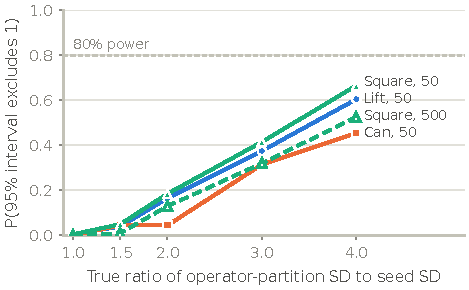
\includegraphics[width=\columnwidth]{fig_power.pdf}
\caption{Power of the preregistered headline procedure (probability that the 95\% interval for $R$ excludes one) as a function of the true ratio, simulated at each task's fitted seed and residual standard deviations with six partitions, three seeds and ten Arm~A seeds.}
\label{fig:power}
\end{figure}

\subsection{Stage 2: the same checkpoints at 500 rollouts}
\label{sec:stage2}
Fig.~\ref{fig:stages} shows the 46 Square checkpoints evaluated at 50 and at 500 rollouts. Three observations follow.

\textbf{A 50-rollout success rate is a poor measurement of a checkpoint.} Across the 46 checkpoints the correlation between the two evaluations is $r=\AgreeR$: the 50-rollout number explains \AgreeRsq\% of the variance of the 500-rollout number. The differences have standard deviation \AgreeSD, matching the binomial expectation of \AgreeExp, and reach \AgreeMax{} points for a single checkpoint. The 50-state set was also \AgreeMean{} points harder on average than the 500-state set, a reminder that results on a small fixed set of initial conditions are conditional on that set.

\textbf{The seed spread shrinks with the noise.} At 500 rollouts the ten-seed standard deviation on Square is \TwoSqASD{} $[\TwoSqASDlo, \TwoSqASDhi]$, against \OneSqASD{} at 50 rollouts, with a floor of \TwoSqBinom.

\textbf{The operator contrast lands on the decision boundary.} The partition standard deviation is \TwoSqBSDp{} in Arm~B and \TwoSqCSDp{} in Arm~C, with equal residuals (\TwoSqBSDe{} and \TwoSqCSDe). The headline ratio is $R=\TwoSqR$ $[\TwoSqRlo, \TwoSqRhi]$, which does not exclude one ($p=\TwoSqRp$). For the control contrast, the preregistered 2000-resample bootstrap gives $D\times10^{3}=\TwoSqD$ $[\TwoSqDlo, \TwoSqDhi]$ with $p=\TwoSqDp$ and Holm-adjusted \TwoSqDpHolm. Because that is within Monte Carlo error of the threshold, we enumerated the bootstrap exactly: there are only 462 distinct resamples of six partitions, so the full distribution can be computed with multinomial weights. The exact interval is $[\TwoSqDExLo, \TwoSqDExHi]$ with $p=\TwoSqDExp$ and Holm-adjusted \TwoSqDExpHolm. The two computations fall on opposite sides of 0.05 by less than 0.002. \emph{We therefore do not claim the contrast.} The point estimates in both stages have the operator partitions varying more than the random ones, and the data are consistent with an operator-composition effect several times larger than the resampling effect, and equally with none that six operators can establish.

\begin{figure*}[t]
\centering
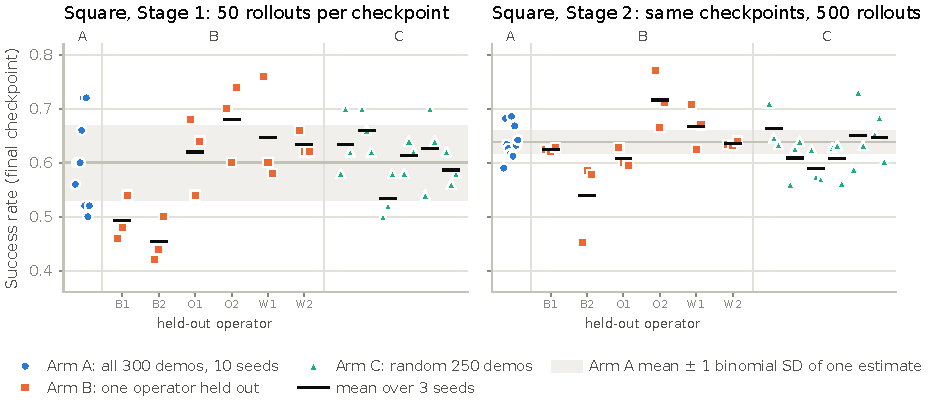
\includegraphics[width=\textwidth]{fig_square_stages.pdf}
\caption{Square: the same 46 final checkpoints evaluated with 50 rollouts (Stage~1, left) and with 500 rollouts on 500 new fixed initial conditions (Stage~2, right). Layout as in Fig.~\ref{fig:arms}. The apparent separation of the two ``better''-operator partitions at 50 rollouts is not present at 500.}
\label{fig:stages}
\end{figure*}

\subsection{Tier labels}
\label{sec:tier}
At 50 rollouts the Square partition means looked like a clear tier effect: holding out either ``better'' operator gave \OneSqDropBOne{} and \OneSqDropBTwo, against \OneSqBMeanHi{} at most for the others, a between-tier share of \OneSqTierShare{} against a null mean of \OneSqTierNull{} (Table~\ref{tab:partitions}). After Stage~1 we recorded, in Amendment~2, that the secondary prediction appeared to be contradicted. At 500 rollouts the pattern is gone. The between-tier share is \TwoSqTierShare, and the mean absolute difference between partitions in the same tier (\TwoSqTierWithin) is as large as between tiers (\TwoSqTierBetween). The partition whose mean moved most, with the first ``better'' operator held out, went from \OneSqDropBOne{} to \TwoSqDropBOne. Amendment~3 withdraws the earlier statement. We make no tier-level claim in either direction; what the comparison shows is that a pattern across six partition means, each a three-seed, 50-rollout average, was strong enough to be written down and did not survive ten times the rollouts.

\begin{table}[t]
\centering
\caption{Square, Arm~B: three-seed mean success rate by held-out operator at 50 and 500 rollouts, and the tier effect sizes. The exact permutation $p$ for the between-tier share is \OneSqTierP{} at 50 rollouts and \TwoSqTierP{} at 500; its minimum attainable value is 0.067.}
\label{tab:partitions}
\resizebox{\columnwidth}{!}{% AUTO-GENERATED by analysis/make_paper_numbers.py. Do not edit.
\begin{tabular}{@{}l cc cc@{}}
\toprule
 & \multicolumn{2}{c}{50 rollouts} & \multicolumn{2}{c}{500 rollouts} \\
\cmidrule(lr){2-3}\cmidrule(l){4-5}
Held-out operator & mean & seed range & mean & seed range \\
\midrule
Better 1 & 0.493 & 0.46--0.54 & 0.624 & 0.62--0.63 \\
Better 2 & 0.453 & 0.42--0.50 & 0.539 & 0.45--0.59 \\
Okay 1 & 0.620 & 0.54--0.68 & 0.607 & 0.59--0.63 \\
Okay 2 & 0.680 & 0.60--0.74 & 0.716 & 0.67--0.77 \\
Worse 1 & 0.647 & 0.58--0.76 & 0.667 & 0.62--0.71 \\
Worse 2 & 0.633 & 0.62--0.66 & 0.635 & 0.63--0.64 \\
\midrule
Between-tier share & \multicolumn{2}{c}{0.94} & \multicolumn{2}{c}{0.43} \\
Null mean share & \multicolumn{2}{c}{0.40} & \multicolumn{2}{c}{0.40} \\
Within-tier $|\Delta|$ & \multicolumn{2}{c}{0.038} & \multicolumn{2}{c}{0.075} \\
Between-tier $|\Delta|$ & \multicolumn{2}{c}{0.124} & \multicolumn{2}{c}{0.071} \\
\bottomrule
\end{tabular}
}
\end{table}

\subsection{What the convention can resolve}
\label{sec:resolve}
Arm~A gives a direct estimate of the run-to-run standard deviation $s$ of a reported number at fixed data. Two methods each reported as the mean of $k$ seeds differ detectably, at a two-sided 95\% level, only if their true difference exceeds roughly
\begin{equation}
\Delta_{\min} \approx 1.96\, s\,\sqrt{2/k}, \qquad s^2 \approx \sigma_{\mathrm{seed}}^2 + \frac{p(1-p)}{n},
\label{eq:mdd}
\end{equation}
where $n$ is the number of rollouts. Table~\ref{tab:resolve} evaluates this for $k=3$. On Square at 50 rollouts the threshold is \OneSqMDD{} points with a normal quantile, and \OneSqMDDt{} with the $t$ quantile appropriate when $s$ is itself estimated from the two three-seed samples. At 500 rollouts it is \TwoSqMDD{} points. These thresholds account for seed and rollout noise only. They do not include the dependence on which demonstrations are in the dataset, for which Arm~C gives a partition standard deviation of \TwoSqCSDp{} on Square at 500 rollouts, nor any operator effect.

\begin{table}[t]
\centering
\caption{Smallest difference between two three-seed means that is distinguishable at 95\% (Eq.~\ref{eq:mdd}), from the Arm~A spread. In parentheses: with the $t$ quantile for 4 degrees of freedom.}
\label{tab:resolve}
\setlength{\tabcolsep}{4pt}
\resizebox{\columnwidth}{!}{% AUTO-GENERATED by analysis/make_paper_numbers.py. Do not edit.
\begin{tabular}{@{}l c ccc c cc@{}}
\toprule
 & & & \multicolumn{2}{c}{floor} & & \multicolumn{2}{c}{min.\ resolvable diff.\ (points)} \\
\cmidrule(lr){4-5}\cmidrule(l){7-8}
Task & $n$ & seed SD & binomial & per-state & Cochran $p$ & paired & unpaired \\
\midrule
Lift & 50 & 0.017 & 0.015 & 0.015 & 0.213 & 2.7 (3.8) & 2.8 (4.0) \\
Can & 50 & 0.023 & 0.032 & 0.032 & 0.855 & 3.7 (5.3) & 5.1 (7.2) \\
Square & 50 & 0.079 & 0.069 & 0.064 & 0.133 & 12.7 (18.0) & 13.4 (18.9) \\
Square & 500 & 0.031 & 0.021 & 0.020 & 0.009 & 5.0 (7.1) & 5.2 (7.3) \\
\bottomrule
\end{tabular}
}
\end{table}

\subsection{Exploratory analyses}
\label{sec:explore}
The following were declared exploratory in Amendment~2 and are not tests of the preregistered claims. (i)~Replacing the denominator of $R$ by the Arm~A spread with the binomial floor removed gives \OneSqRCorr{} on Square at 50 rollouts and \TwoSqRCorr{} at 500, but the correction is unstable: in \OneSqRCorrFloorFrac\% and \TwoSqRCorrFloorFrac\% of resamples respectively the Arm~A spread is at or below the floor and the ratio is undefined, and on Can it is undefined at the point estimate. (ii)~The exact $F$-test for a partition component gives $p=\OneSqBFp$ in Arm~B against \OneSqCFp{} in Arm~C on Square at 50 rollouts, and \TwoSqBFp{} against \TwoSqCFp{} at 500; on Lift and Can no test is below 0.05. (iii)~The difference between partitions that hold out a ``better'' operator and the rest is \OneSqDropDiff{} points at 50 rollouts and \TwoSqDropDiff{} at 500 on Square. These are consistent with a partition effect in Arm~B on Square, and none of them changes the status of the preregistered contrasts.

\section{Discussion and Recommendations}
\label{sec:recs}
The hypothesis we registered was about operators. The clearest finding is about rollouts. Three-seed, 50-rollout reporting on these benchmarks produces an uncertainty that is dominated by binomial evaluation noise on two of three tasks, and a point estimate that, on the third, is a weak proxy for the same checkpoint's success rate under a larger evaluation. The published statement that motivated this study, that comparisons separated by a few points are not resolvable from the reported statistic, is supported on Square by Table~\ref{tab:resolve}, for a reason more elementary than the one we proposed.

For the operator question, both stages give the same ordering of point estimates on Square, with operator partitions varying more than size-matched random partitions, and neither stage establishes it. We regard this as an open question that six operators cannot settle at any rollout count: at 500 rollouts the preregistered procedure still has only \TwoSqPowTwo\% power at a true ratio of two. A dataset with more operators is required.

We recommend the following for results on these and similar benchmarks.
\begin{enumerate}
\item \textbf{Report the binomial standard error next to the seed standard deviation.} A seed standard deviation at or below $\sqrt{p(1-p)/n}$ does not indicate a stable method; it indicates that the evaluation cannot see the seed effect.
\item \textbf{Evaluate with enough rollouts for the task's success band.} Near 60\% success, 50 rollouts give a standard error of 7 points per checkpoint; 500 give 2. Rollouts in simulation are cheap relative to training, and Eq.~(\ref{eq:mdd}) states what a given budget can resolve.
\item \textbf{Fix, store and publish the initial conditions,} including the scene model where the simulator randomises it, and report results on a set large enough that conclusions are not conditional on it.
\item \textbf{Evaluate a checkpoint chosen without the evaluation rollouts.} We used the final one.
\item \textbf{State the composition of the training set} when subsets of a multi-operator dataset are used, and do not read structure, such as a tier effect, from a handful of low-rollout partition means.
\item \textbf{Release per-rollout outcomes.} They make every analysis above reproducible by others.
\end{enumerate}

\section{Limitations}
Six operators per task is the binding limitation; it sets the power of every operator-level test here. The study uses one architecture, low-dimensional observations, one training length, simulation only, and one benchmark family. Arms~B and~C have three seeds per partition. Partitions within an arm overlap heavily, so the partition effects are not independent draws from a population, and the random-effects model is an approximation; Arm~C shares that structure, which is why the contrast with it, rather than the absolute component, is the meaningful quantity. Stage~2 was designed after Stage~1 results were known and reuses its checkpoints. The exact bootstrap enumeration was added after the Stage~2 contrast was seen to be at the boundary; it changes no statistic, but it is why two $p$-values are reported, and we adopted the more conservative reading. Operator labels are those released with the dataset, and no operator-level covariates exist. Success rates on a fixed set of initial conditions are conditional on that set.

\section{Conclusion}
We preregistered the claim that operator composition contributes more variance than training seed on the robomimic Multi-Human benchmarks, ran 138 training runs with a matched random control, and did not confirm it. The experiment was underpowered for that claim by the number of operators, not by compute. It was well powered for a different conclusion: the conventional three-seed, 50-rollout statistic mostly measures evaluation noise on Lift and Can, cannot resolve differences smaller than about \OneSqMDD{} points on Square, and was sufficient to produce a tier pattern that a tenfold larger evaluation did not reproduce. Reporting practice on these benchmarks should change accordingly, and the operator question should be revisited on data with more demonstrators.

\section*{Reproducibility}
The repository contains the preregistration and amendments with their commit history, the pinned environment, dataset checksums, the immutable partition files, the stored initial conditions, the training and evaluation queue, per-run and per-rollout CSV files for both stages (6{,}900 and 23{,}000 rollouts), and the scripts that regenerate every number, table and figure in this paper from those files.

\IfFileExists{IEEEtran.bst}{\bibliographystyle{IEEEtran}}{\bibliographystyle{unsrt}}
\bibliography{refs}

\end{document}
